%%%%%%%%%%%%%%%%%%%%%%%%%%%%%%%%%%%%%%%%%
% Beamer Presentation
% LaTeX Template
% Version 2.0 (March 8, 2022)
%
% This template originates from:
% https://www.LaTeXTemplates.com
%
% Author:
% Vel (vel@latextemplates.com)
%
% License:
% CC BY-NC-SA 4.0 (https://creativecommons.org/licenses/by-nc-sa/4.0/)
%
%%%%%%%%%%%%%%%%%%%%%%%%%%%%%%%%%%%%%%%%%

%----------------------------------------------------------------------------------------
%	PACKAGES AND OTHER DOCUMENT CONFIGURATIONS
%----------------------------------------------------------------------------------------

\documentclass[
	11pt, % Set the default font size, options include: 8pt, 9pt, 10pt, 11pt, 12pt, 14pt, 17pt, 20pt
	%t, % Uncomment to vertically align all slide content to the top of the slide, rather than the default centered
	aspectratio=169, % Uncomment to set the aspect ratio to a 16:9 ratio which matches the aspect ratio of 1080p and 4K screens and projectors
]{beamer}

%\graphicspath{{Images/}{./}} % Specifies where to look for included images (trailing slash required)

\usepackage{booktabs} % Allows the use of \toprule, \midrule and \bottomrule for better rules in tables
\usepackage{kotex}
\usepackage[backend=biber,style=authoryear]{biblatex} % 참고문헌 관련 설정
\addbibresource{references.bib} % BibTeX 파일 경로

%----------------------------------------------------------------------------------------
%	SELECT LAYOUT THEME
%----------------------------------------------------------------------------------------

% Beamer comes with a number of default layout themes which change the colors and layouts of slides. Below is a list of all themes available, uncomment each in turn to see what they look like.


\usetheme{CambridgeUS}

%----------------------------------------------------------------------------------------
%	SELECT COLOR THEME
%----------------------------------------------------------------------------------------

% Beamer comes with a number of color themes that can be applied to any layout theme to change its colors. Uncomment each of these in turn to see how they change the colors of your selected layout theme.

\usecolortheme{dolphin}

%----------------------------------------------------------------------------------------
%	SELECT FONT THEME & FONTS
%----------------------------------------------------------------------------------------

% Beamer comes with several font themes to easily change the fonts used in various parts of the presentation. Review the comments beside each one to decide if you would like to use it. Note that additional options can be specified for several of these font themes, consult the beamer documentation for more information.

\usefonttheme{default} % Typeset using the default sans serif font

%------------------------------------------------

\usepackage{mathptmx} % Use the Times font for serif text
%\usepackage{palatino} % Use the Palatino font for serif text

%\usepackage{helvet} % Use the Helvetica font for sans serif text
\usepackage[default]{opensans} % Use the Open Sans font for sans serif text
%\usepackage[default]{FiraSans} % Use the Fira Sans font for sans serif text
%\usepackage[default]{lato} % Use the Lato font for sans serif text

\usepackage[ruled,vlined]{algorithm2e}
\usepackage{algorithmicx}
\usepackage{multicol}

%----------------------------------------------------------------------------------------
%	SELECT INNER THEME
%----------------------------------------------------------------------------------------

% Inner themes change the styling of internal slide elements, for example: bullet points, blocks, bibliography entries, title pages, theorems, etc. Uncomment each theme in turn to see what changes it makes to your presentation.

%\useinnertheme{default}
\useinnertheme{circles}

%----------------------------------------------------------------------------------------
%	Other Change
%----------------------------------------------------------------------------------------

% Change standard block width
\addtobeamertemplate{block begin}{%
    \setlength{\textwidth}{0.9\textwidth}
}{}


%----------------------------------------------------------------------------------------
%	PRESENTATION INFORMATION
%----------------------------------------------------------------------------------------

\title[OPF using Matpower and Pyomo]{Optimal Power Flow \\ using Matpower and Pyomo} % The short title in the optional parameter appears at the bottom of every slide, the full title in the main parameter is only on the title page

%\subtitle{Optional Subtitle} % Presentation subtitle, remove this command if a subtitle isn't required

\author[Woong Ko]{Prof. Woong Ko} % Presenter name(s), the optional parameter can contain a shortened version to appear on the bottom of every slide, while the main parameter will appear on the title slide

\institute[CWNU]{Changwon National University \\ \smallskip \textit{kwoong@changwon.ac.kr}} % Your institution, the optional parameter can be used for the institution shorthand and will appear on the bottom of every slide after author names, while the required parameter is used on the title slide and can include your email address or additional information on separate lines

\date[\today]{\today} % Presentation date or conference/meeting name, the optional parameter can contain a shortened version to appear on the bottom of every slide, while the required parameter value is output to the title slide

%----------------------------------------------------------------------------------------

\begin{document}

%----------------------------------------------------------------------------------------
%	TITLE SLIDE
%----------------------------------------------------------------------------------------

\begin{frame}
	\titlepage % Output the title slide, automatically created using the text entered in the PRESENTATION INFORMATION block above
\end{frame}

%----------------------------------------------------------------------------------------
%	TABLE OF CONTENTS SLIDE
%----------------------------------------------------------------------------------------

% The table of contents outputs the sections and subsections that appear in your presentation, specified with the standard \section and \subsection commands. You may either display all sections and subsections on one slide with \tableofcontents, or display each section at a time on subsequent slides with \tableofcontents[pausesections]. The latter is useful if you want to step through each section and mention what you will discuss.

\begin{frame}[allowframebreaks]
	\frametitle{Table of Contents} % Slide title, remove this command for no title
	
	\tableofcontents % Output the table of contents (all sections on one slide)
	%\tableofcontents[pausesections] % Output the table of contents (break sections up across separate slides)
\end{frame}

%----------------------------------------------------------------------------------------
%	PRESENTATION BODY SLIDES
%----------------------------------------------------------------------------------------

\section{Background} % Sections are added in order to organize your presentation into discrete blocks, all sections and subsections are automatically output to the table of contents as an overview of the talk but NOT output in the presentation as separate slides

%------------------------------------------------

\subsection{Optimal Power Flow?}

\begin{frame}
	\frametitle{Optimal Power Flow?}
	
	The \alert{optimal power flow(OPF)} can integrate the compuation of power flow and operational problems (such as economic dispatch and unit commitment) subject to the power system's pysical and electrical constraints.

	\bigskip % Vertical whitespace
	
	% Quote example
	\begin{quote}
		The optimal power flow (OPF) integrates the computation of power flow and economic dispatch subject to the system's physical and electrical constraints \ldots \parencite{Ali_2024}
	\end{quote}
	
	\bigskip % Vertical whitespace
	
	
\end{frame}


%------------------------------------------------

\begin{frame}
	\frametitle{Optimal Power Flow?}

	\begin{itemize}
	\item Optimal power flow = \color{blue}{Optimization problem} + \alert{Power flow}
	\end{itemize}

	\begin{columns}
	
	\begin{column}{0.5\textwidth}
	\begin{block}{\color{blue}{Optimization problem}}
		\begin{itemize}
		\item Find the optimal variables satisfying the objective function
		\item Example: 
			\begin{align*} 
				\min_{x\in D} \quad & f(x) \\
				\text{subject to} \quad & g_{i}(x) \leq 0, \quad i=1,...,m \\
				& h_{j}(x) = 0, \quad j=1,...,r
			\end{align*}
		\end{itemize}
	\end{block}
	\end{column}

	\begin{column}{0.5\textwidth}
	\begin{block}{\alert{Power flow}}
		\begin{itemize}
		\item Find the variables satisfying the power flow equation
		\item Example:
			\begin{align*} 
				P_{i} = \left|V_{i}\right| \sum_{\forall j} \left|V_{j}\right|
				& \left[
				G_{ij}\cos \left(\theta_{i} - \theta_{j} \right) \right.\\
				&\left.+ B_{ij}\sin \left(\theta_{i} - \theta_{j} \right) \right]
			\end{align*}
		\end{itemize}
	\end{block}
	\end{column}

	\end{columns}

\end{frame}


%------------------------------------------------

\begin{frame}
	\frametitle{Optimal Power Flow?}
	\framesubtitle{Optimization problem and power flow problem} % Optional subtitle
	
	\begin{itemize}
		\item \color{blue}{Optimization problem}
		\begin{itemize}
			\item Solve the problem based on the optimization techniques\\ 
			(convex, branch and bound, etc)
				\begin{itemize}
				\item 조건에 따라 해가 존재하지 않을 수 있음
				\item Variables: Generator status, reactive/active power, voltage magnitude/phase, etc
			\end{itemize}
		\end{itemize}
	\end{itemize}

	\begin{itemize}
		\item \alert{Power flow}
		\begin{itemize}
			\item Solve the problem based on finding the solution on multiple equations \\
			(Newton Raphson, Gauss-Seidel)
				\begin{itemize}
				\item 초기값 혹은 계통에 문제가 없지 않은 이상 해는 존재
				\item Variables: Reactive/active power, voltage magnitude/phase
			\end{itemize}
		\end{itemize}
	\end{itemize}

		\begin{itemize}
		\item Optimization problem + power flow
		\begin{itemize}
			\item 다양한 목적함수를 가지며 제약조건으로 power flow를 갖는 최적화 문제
				\begin{itemize}
				\item 손실 최소화, 비용 최소화, 이익 최대화 등
			\end{itemize}
		\end{itemize}
	\end{itemize}
	
\end{frame}


%------------------------------------------------

\begin{frame}
	\frametitle{Optimal Power Flow?}
	\framesubtitle{Problems defined by variable type} % Optional subtitle
	
	\begin{itemize}
		\item Linear programming (LP)
		\begin{itemize}
			\item 모든 목적함수와 제약조건이 선형화 되어있는 상황이며, 발전량과 전압의 크기/위상 등 continuous variable 을 결정하는 문제
			\item Cplex, Gurobi 등 solver 이용 가능
			\item Global optimum 을 찾을 수 있으나 비선형방정식을 선형방정식으로 바꿔야 함
		\end{itemize}
		
		\item Mixed integer linear programming (MILP)
		\begin{itemize}
			\item 모든 목적함수와 제약조건이 선형화 되어있고, 이진변수(0 or 1)이 존재하는 최적화 문제
			\item 이진변수는 발전기의 On/Off, ESS의 충방전 Mode 선택 등 다양한 변수가 존재
			\item Cplex, Gurobi 등 solver 이용 가능
			\item Global optimum 을 찾을 수 있으나 비선형방정식을 선형방정식으로 바꿔야 함
			\item Solver가 이진변수를 relaxation (이진 변수를 연속 변수로 완화) 하는 것으로 알려짐
		\end{itemize}

	\end{itemize}
	
\end{frame}


%------------------------------------------------

\begin{frame}
	\frametitle{Optimal Power Flow?}
	\framesubtitle{Problems defined by variable type} % Optional subtitle
	
	\begin{itemize}
		\item Mixed integer nonlinear programming (MINLP)
		\begin{itemize}
			\item 목적함수와 제약조건에 비선형 방정식 등이 포함된 최적화 문제
			\item 이진변수, 연속변수 등 다양한 변수와 함께 전력방정식이 그대로 포함될 수 있음
			\item 문제를 선형함수로 변환하지 않아도 되기 때문에 해가 구해진다면 정확한 해일 가능성이 높음
			\item 하지만, solver 성능에 따라 문제가 풀리지 않는 경우들이 대부분
			\item Local optimum 과 global optimum 이 같지 않을 수 있음을 항상 고민해야 함
			\item Knitro 등의 solve를 사용

		\end{itemize}
		
		\item Meta heuristic
		\begin{itemize}
			\item 비선형 방정식 등이 포함된 최적화 문제이나 문제 해결을 위해 다양한 방법을 활용하는 기법
			\item 기본적으로 변수에 여러 값들을 대입하면서 구하는 문제 해결 방법이지만, 다양한 알고리즘이 사용됨
			\item Genetic algorithm, particle swarm optimization, harmony search 등의 방법이 사용됨
			\item Pygmo 등으로 이용할 수 있으며, matlab 을 이용하는 것이 일반적임

		\end{itemize}

	\end{itemize}
	
\end{frame}


%------------------------------------------------

\begin{frame}
	\frametitle{Optimal Power Flow?}
	\framesubtitle{How to solve?} % Optional subtitle
	
	\begin{itemize}
		\item 문제 해결의 기본 방향
		\begin{itemize}
			\item 최적화 문제를 처음 해결하는 상황이라면, 목적함수와 제약조건의 방정식을 그대로 이용할 수 있는 MINLP와 meta heuristic 방법을 이용하는 것도 방법임
			\item 위 방법을 이용한 이후에는 relaxation 등을 통하여 MILP, LP 문제로 바꾸어 해결하는 방안을 고민할 수 있음
		\end{itemize}
		
		\item 문제 유형별 사용 Solver
		\begin{itemize}
			\item LP, MILP: Pyomo 에서 cplex, gurobi 등을 연계
			\item MINLP: Pyomo 에서 knitro 등을 연계
			\item Meta heuristic: Pyomo 에서는 해결하지 못하며, Pygmo 등을 사용
		\end{itemize}

	\end{itemize}
	
\end{frame}

%------------------------------------------------

\subsection{Previous studies}

\begin{frame}
	\frametitle{Previous studies}
	\framesubtitle{Typical optimal power flow problem}
	Minimize the loss in the overall system\parencite{5982115}.

	\begin{figure}
		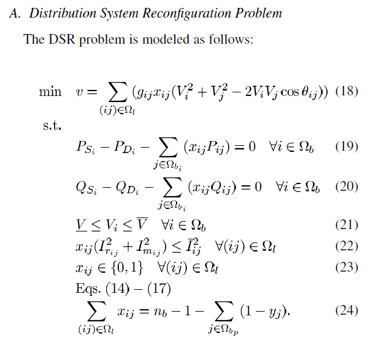
\includegraphics[width=2.5 in,keepaspectratio]{typ_opf.png}
	\end{figure}
	
	
\end{frame}

%------------------------------------------------

\begin{frame}
	\frametitle{Previous studies}
	\framesubtitle{Typical optimal power flow problem}
	\begin{itemize}
		\item Objective function: Minimize the loss
		\begin{align*}
			\min \quad v= \sum_{(ij) \in \Omega_{l} }
			(g_{ij}(\left|V_{i}\right|^{2}+\left|V_{j}\right|^{2}-2\left|V_{i}\right| \left|V_{j}\right|\cos\theta_{ij}))
		\end{align*}
	\end{itemize}
\end{frame}


%------------------------------------------------


\begin{frame}
	\frametitle{Previous studies}
	\framesubtitle{Typical optimal power flow problem}
	
	Equality constraints:
	\begin{itemize}
	\item Balance
		\begin{itemize}
			\item Active power
				\begin{align*}
					&P_{S_{i}}-P_{D_{i}}-\sum_{j \in \Omega_{b_{i}}} P_{ij} = 0\\
					&(P_{ij}=-\left|V_{i} \right|^{2}G_{ij}+\left|V_{i} \right|\left|V_{j} \right|(G_{ij}\cos\theta_{ij} + B_{ij}\sin\theta_{ij}))
				\end{align*}

			\item Reactive power
				\begin{align*}
					&Q_{S_{i}}-Q_{D_{i}}-\sum_{j \in \Omega_{b_{i}}} Q_{ij} = 0\\
					&Q_{ij}=\left|V_{i} \right|^{2}B_{ij}+\left|V_{i} \right|\left|V_{j} \right|(G_{ij}\sin\theta_{ij} - B_{ij}\sin\theta_{ij})
				\end{align*}
		\end{itemize}

	\end{itemize}
	
	
\end{frame}


%------------------------------------------------

\begin{frame}
	\frametitle{Typical optimal power flow problem}
	\framesubtitle{Constraints} % Optional subtitle
	
	Inequality constraints:
	\begin{itemize}
	\item Operation condition
		\begin{itemize}
			\item Voltage
				\begin{align*}
					\underline{\left| V_{i} \right|} \leq \left| V_{i} \right| \leq \overline{\left| V_{i} \right|}
				\end{align*}

			\item Line rating
				\begin{align*}
					I^{2}_{real,ij}+I^{2}_{imag,ij} \leq \overline{I^{2}_{ij}}
				\end{align*}
		\end{itemize}

	\end{itemize}
	
	
\end{frame}

%------------------------------------------------

\subsection{Purpose and Objectives}

\begin{frame}
	\frametitle{Our main objective is to...}
	
	\begin{itemize}
		\item Formulate the objective function and constraints of the Optimal Power Flow (OPF) problem.
		\item Implement the formulated objective function and constraints using Matpower and Pyomo.
		\item Derive simulation results of the implemented model on a 33-bus test system.
	\end{itemize}
	
	
\end{frame}

%------------------------------------------------
\section{Formulation}

\begin{frame}[plain] % The optional argument 'plain' hides the headline and footline
	\begin{center}
		{\Huge Formulation}
		
		\bigskip\bigskip % Vertical whitespace
		
	\end{center}
\end{frame}

%------------------------------------------------

\subsection{Overview}

\begin{frame}
	\frametitle{Overview}

	\begin{columns}
	
		\begin{column}{0.5\textwidth}
			\begin{itemize}
				\item Nomenclature: Slide~\ref{frame:Nomenclature}
				\item At glance...: Slide~\ref{frame:atglance}
				\item Objective function: Slide~\ref{frame:objfunc}
				\item Constraints and expressions: Slide~\ref{frame:constraints}
					\begin{itemize}
						\item Load balance
						\item Power and voltage
						\item Current
					\end{itemize}
			\end{itemize}
		\end{column}

		\begin{column}{0.5\textwidth}
			Optimization problem is formulated as:
			\begin{enumerate}
				\item Objective function:
				\[
					\text{minimize (or maximize) } f(\mathbf{x})
				\]
				\item Constraints:
				\[
					g(\mathbf{x}) \leq 0, \quad h(\mathbf{x}) = 0
				\]
				\item Functions in the objective and constraints:
				\[
					f(\mathbf{x}), \quad g(\mathbf{x}), \quad h(\mathbf{x})
				\]
			\end{enumerate}
		\end{column}

	\end{columns}

\end{frame}

%------------------------------------------------

\subsection{Nomenclature}

\begin{frame}
	\frametitle{Nomenclature}
	\label{frame:Nomenclature}
	\framesubtitle{Sets, indices, parameters}

	\begin{columns}
	
		\begin{column}{0.5\textwidth}
			
			\begin{itemize}
			\item Indices
			\end{itemize}

			\begin{tabular}{ll}
				$i,j$ & Index of bus \\
				$l$ & Index of line \\
			\end{tabular}
			
			\bigskip
			
			\begin{itemize}
			\item Sets
			\end{itemize}

			\begin{tabular}{ll}
				$\Omega_{l}$ & Set of lines \\
				$\Omega_{b}$ & Set of buses\\
				$\Omega_{b_{i}}$ & \begin{tabular}[l]{@{}l@{}}Set of connected buses \\ in the bus $i$\end{tabular}\\
				$\Omega_{b_{g}}$ & \begin{tabular}[l]{@{}l@{}}Set of generation buses \\ ($\Omega_{b_{g}}$ $\subset$ $\Omega_{b}$)\end{tabular}\\
			\end{tabular}

		\end{column}

		\begin{column}{0.5\textwidth}
			\begin{itemize}
			\item Parameters or constants
			\end{itemize}

			\begin{tabular}{ll}
				$Z_{ij}$, $Y_{ij}$ & \begin{tabular}[l]{@{}l@{}}Impedance and \\admittance of line $ij$\\(from bus $i$ to bus $j$)\end{tabular} \\
				$G_{ij}$, $B_{ij}$ & \begin{tabular}[l]{@{}l@{}}Conductance and \\susceptance of line $ij$\\(from bus $i$ to bus $j$)\end{tabular} \\
				$baseMVA$ & Value of base MVA \\
				$\overline{V}$, $\underline{V}$ & \begin{tabular}[l]{@{}l@{}}Maximum and minimum \\voltage magnitude\end{tabular}\\
				$\overline{I}_{ij}$ & \begin{tabular}[l]{@{}l@{}}Maximum current \\ flow limit of line $ij$\end{tabular}\\
			\end{tabular}

		\end{column}

	\end{columns}

\end{frame}

%------------------------------------------------

\begin{frame}
	\frametitle{Nomenclature}
	\framesubtitle{Sets, indices, parameters}

	\begin{columns}

		\begin{column}{0.5\textwidth}
			\begin{itemize}
			\item Parameters or constants (Continued)
			\end{itemize}

			\begin{tabular}{ll}
				$P_{D_{i}}$, $Q_{D_{i}}$ & \begin{tabular}[l]{@{}l@{}}Active and reactive \\ power demand at bus $i$\end{tabular}\\
				$\overline{P}_{G_{i}}$, $\underline{P}_{G_{i}}$ & \begin{tabular}[l]{@{}l@{}}Maximum and minimum \\active power from generator \\ at bus $i$\end{tabular}\\
				$\overline{Q}_{G_{i}}$, $\underline{Q}_{G_{i}}$ & \begin{tabular}[l]{@{}l@{}}Maximum and minimum \\reactive power from \\ generator at bus $i$\end{tabular}\\
			\end{tabular}

		\end{column}

		\begin{column}{0.5\textwidth}
			\begin{itemize}
			\item Functions
			\end{itemize}

			\begin{tabular}{ll}
				$P_{ij}$, $Q_{ij}$& \begin{tabular}[l]{@{}l@{}}Active and reactive \\ power flow of line $ij$\end{tabular}\\
				$I_{r_{ij}}$, $I_{Im_{ij}}$& \begin{tabular}[l]{@{}l@{}}Real and Imaginary \\ current flow of line $ij$\end{tabular}\\
				$P^{lineloss}_{l}$& \begin{tabular}[l]{@{}l@{}}Active line loss of line $l(ij)$\end{tabular}\\
			\end{tabular}

		\end{column}

	\end{columns}

\end{frame}

%------------------------------------------------

\begin{frame}
	\frametitle{Nomenclature}
	\framesubtitle{Variables}

	\begin{columns}

	
		\begin{column}{0.5\textwidth}
			\begin{itemize}
			\item Varaibles
			\end{itemize}

			\begin{tabular}{ll}
				$\left|\dot{V}_{i} \right|$ & Voltage magnitude in bus $i$ \\
				$\theta_{i}$ & Voltage phase angle in bus $i$  \\
				$P_{G_{i}}$, $Q_{G_{i}}$ & \begin{tabular}[l]{@{}l@{}}Active and reactive power \\from generator at bus $i$\end{tabular}\\
			\end{tabular}

			\bigskip

		\end{column}

	\end{columns}

\end{frame}

%------------------------------------------------

\subsection{At glance...}

\begin{frame}
	\frametitle{At glance...}
	\label{frame:atglance}
	
	Objective function: Eq.~\eqref{eq:obj}
	\begin{align*}
		\min{ \sum_{\forall i,j} {[-G_{ij}(\left|\dot{V}_{i} \right|^2 + \left|\dot{V}_{j} \right|^2) + 2G_{ij}\left|\dot{V}_{i} \right|\left|\dot{V}_{j} \right|\cos\left(\theta_{i}-\theta_{j} \right) ]} }
	\end{align*}

	Constraints: Eqs.~\eqref{eq:cons_load_bal_P},\eqref{eq:cons_load_bal_Q},\eqref{eq:cons_power_P},\eqref{eq:cons_power_Q},\eqref{eq:cons_voltage},\eqref{eq:cons_slack},\eqref{eq:cons_current}
	\begin{columns}
		\begin{column}{0.5\textwidth}
			\begin{align*}
				s.t. \quad
				P_{G_{i}} - P_{D_{i}} = \sum_{j \in \Omega_{b_{i}}}(P_{ij})  \quad \forall i \in \Omega_{b}\\
				Q_{G_{i}} - Q_{D_{i}} = \sum_{j \in \Omega_{b_{i}}}(Q_{ij})  \quad \forall i \in \Omega_{b}\\
				\underline{P}_{G_{i}} \leq P_{G_{i}} \leq \overline{P}_{G_{i}}  \quad \forall i \in \Omega_{b}\\
				\underline{Q}_{G_{i}} \leq Q_{G_{i}} \leq \overline{Q}_{G_{i}}  \quad \forall i \in \Omega_{b}\\
			\end{align*}
		\end{column}

		\begin{column}{0.5\textwidth}
			\begin{align*}
				\underline{V} \leq \left|\dot{V}_{i} \right| \leq \overline{V}  \quad \forall i \in \Omega_{b}\\
				\theta_{i} = \left\{ \begin{array}{cl}
							0 & : \ \text{Bus } i \text{ is slack,} \\
							\text{free} & : \ \text{Otherwise.}
							\end{array} \right.\\
				I_{r_{ij}}^{2}+ I_{Im_{ij}}^{2} \leq \overline{I}_{ij}^{2} \quad   \forall l(ij) \in \Omega_{l}\\
			\end{align*}
		\end{column}
	\end{columns}
	
\end{frame}

%------------------------------------------------

\begin{frame}
	\frametitle{At glance...}
	
	Functions or expressions: Eq.~\eqref{eq:expr_loss}, \eqref{eq:expr_p_flow_ij}, \eqref{eq:expr_p_flow_ji}
	\begin{align*}
		[-G_{ij}(\left|\dot{V}_{i} \right|^2 + \left|\dot{V}_{j} \right|^2) + 2G_{ij}\left|\dot{V}_{i} \right|\left|\dot{V}_{j} \right|\cos\left(\theta_{i}-\theta_{j} \right) ] =P_{l}^{line loss}= P_{ij} + P_{ji} \quad \quad \forall l(ij) \in \Omega_{l}
	\end{align*}

	\begin{align*}
		\begin{split}
		P_{ij} = &-G_{ij} \left|\dot{V}_{i} \right| \left|\dot{V}_{i} \right| 
		+ G_{ij} \left|\dot{V}_{i} \right| \left|\dot{V}_{j} \right| \cos\left(\theta_{i}-\theta_{j} \right) \\
		&+ B_{ij} \left|\dot{V}_{i} \right| \left|\dot{V}_{j} \right| \sin\left(\theta_{i}-\theta_{j} \right) 
		\quad \quad \forall l \in \Omega_{l} \quad \text{or} \quad \forall (ij) \in \Omega_{l}
		\end{split}
	\end{align*}

	\begin{align*}
		\begin{split}
		P_{ji}=&-G_{ij} \left|\dot{V}_{j} \right| \left|\dot{V}_{j} \right| 
		+ G_{ij} \left|\dot{V}_{i} \right| \left|\dot{V}_{j} \right| \cos\left(\theta_{i}-\theta_{j} \right)\\
		&- B_{ij} \left|\dot{V}_{i} \right| \left|\dot{V}_{j} \right| \sin\left(\theta_{i}-\theta_{j} \right)
		\quad \quad \forall l \in \Omega_{l} \quad \text{or} \quad \forall (ij) \in \Omega_{l}
		\end{split}
	\end{align*}

	
\end{frame}

%------------------------------------------------

\begin{frame}
	\frametitle{At glance...}
	
	Functions or expressions(Continued): Eq.~\eqref{eq:expr_q_flow_ij}, \eqref{eq:expr_i_re}, \eqref{eq:expr_i_imag}
	
	\begin{align*}
		\begin{split}
			Q_{ij}=&B_{ij}\left\lvert \dot{V}_{i}\right\rvert^{2} + G_{ij}\left\lvert \dot{V}_{i}\right\rvert\left\lvert \dot{V}_{j}\right\rvert \sin{\left(\theta_{i}-\theta_{j}\right)} \\
			&- B_{ij}\left\lvert \dot{V}_{i}\right\rvert\left\lvert \dot{V}_{j}\right\rvert \cos{\left(\theta_{i}-\theta_{j}\right)}  \quad   \forall l \in \Omega_{l} \quad \text{or} \quad \forall (ij) \in \Omega_{l}
		\end{split}
	\end{align*}
	
	\begin{align*}
		\begin{split}
	 		I_{r_{ij}} = &-G_{ij}\left\lvert \dot{V}_{i} \right\rvert \cos{\theta_{i}} + B_{ij}\left\lvert \dot{V}_{i} \right\rvert \sin{\theta_{i}} \\
					&+ G_{ij}\left\lvert \dot{V}_{j} \right\rvert \cos{\theta_{j}} - B_{ij}\left\lvert \dot{V}_{j} \right\rvert \sin{\theta_{j}} \quad \forall l \in \Omega_{l} \quad \text{or} \quad \forall (ij) \in \Omega_{l}
		\end{split}
	\end{align*}

	\begin{align*}
		\begin{split}
	 		I_{Im_{ij}} = &-B_{ij}\left\lvert \dot{V}_{i} \right\rvert \cos{\theta_{i}} - G_{ij}\left\lvert \dot{V}_{i} \right\rvert \sin{\theta_{i}} \\
			&+ B_{ij}\left\lvert \dot{V}_{j} \right\rvert \cos{\theta_{j}} + G_{ij}\left\lvert \dot{V}_{j} \right\rvert \sin{\theta_{j}} \quad \forall l \in \Omega_{l} \quad \text{or} \quad \forall (ij) \in \Omega_{l}
		\end{split}
	\end{align*}

	
\end{frame}

%------------------------------------------------



\subsection{Objective function}

\begin{frame}
	\frametitle{Objective function}
	\label{frame:objfunc}
	\begin{align}
	\label{eq:obj}
		\min{ \sum_{\forall i,j} {[-G_{ij}(\left|\dot{V}_{i} \right|^2 + \left|\dot{V}_{j} \right|^2) + 2G_{ij}\left|\dot{V}_{i} \right|\left|\dot{V}_{j} \right|\cos\left(\theta_{i}-\theta_{j} \right) ]} }
	\end{align}

	\begin{align}
	\label{eq:expr_loss}
		[-G_{ij}(\left|\dot{V}_{i} \right|^2 + \left|\dot{V}_{j} \right|^2) + 2G_{ij}\left|\dot{V}_{i} \right|\left|\dot{V}_{j} \right|\cos\left(\theta_{i}-\theta_{j} \right) ] =P_{l}^{line loss}= P_{ij} + P_{ji} \quad \quad \forall l(ij) \in \Omega_{l}
	\end{align}

	\begin{align}
	\label{eq:expr_p_flow_ij}
		\begin{split}
		P_{ij} = &-G_{ij} \left|\dot{V}_{i} \right| \left|\dot{V}_{i} \right| 
		+ G_{ij} \left|\dot{V}_{i} \right| \left|\dot{V}_{j} \right| \cos\left(\theta_{i}-\theta_{j} \right) \\
		&+ B_{ij} \left|\dot{V}_{i} \right| \left|\dot{V}_{j} \right| \sin\left(\theta_{i}-\theta_{j} \right) 
		\quad \quad \forall l \in \Omega_{l} \quad \text{or} \quad \forall (ij) \in \Omega_{l}
		\end{split}
	\end{align}

	\begin{align}
	\label{eq:expr_p_flow_ji}
		\begin{split}
		P_{ji}=&-G_{ij} \left|\dot{V}_{j} \right| \left|\dot{V}_{j} \right| 
		+ G_{ij} \left|\dot{V}_{i} \right| \left|\dot{V}_{j} \right| \cos\left(\theta_{i}-\theta_{j} \right)\\
		&- B_{ij} \left|\dot{V}_{i} \right| \left|\dot{V}_{j} \right| \sin\left(\theta_{i}-\theta_{j} \right)
		\quad \quad \forall l \in \Omega_{l} \quad \text{or} \quad \forall (ij) \in \Omega_{l}
		\end{split}
	\end{align}


\end{frame}

%------------------------------------------------

\begin{frame}
	\frametitle{Objective function (Derivation of the formula)}
	\framesubtitle{Sending flow} % Optional subtitle

	\begin{align*}
		\dot{S}_{ij}=&\dot{V}_{i}\dot{I}_{ij}^{*} = \dot{V}_{i}\left( \frac{\dot{V}_{i}-\dot{V}_{j}}{\dot{Z}_{ij}}   \right) ^{*}  \\
		=&\dot{V}_{i}\frac{\dot{V}_{i}^{*}}{\dot{Z}_{ij}^{*}} - \dot{V}_{i}\frac{\dot{V}_{j}^{*}}{\dot{Z}_{ij}^{*}} \quad \left(Y_{ij} =-\frac{1}{Z_{ij}} = G_{ij}+jB_{ij}\right) \\
		=&\left\lvert \dot{V}_{i}\right\rvert^{2} \left(-G_{ij}+jB_{ij}\right) - \left\lvert \dot{V}_{i}\right\rvert\left\lvert \dot{V}_{j}\right\rvert e^{j\left(\theta_{i}-\theta_{j}\right) } \left(-G_{ij}+jB_{ij}\right)\\
		=&-G_{ij}\left\lvert \dot{V}_{i}\right\rvert^{2} + G_{ij}\left\lvert \dot{V}_{i}\right\rvert\left\lvert \dot{V}_{j}\right\rvert \cos{\theta_{ij}} + B_{ij}\left\lvert \dot{V}_{i}\right\rvert\left\lvert \dot{V}_{j}\right\rvert \sin{\theta_{ij}}  \\
		 &+j\left( B_{ij}\left\lvert \dot{V}_{i}\right\rvert^{2} + G_{ij}\left\lvert \dot{V}_{i}\right\rvert\left\lvert \dot{V}_{j}\right\rvert \sin{\theta_{ij}} - B_{ij}\left\lvert \dot{V}_{i}\right\rvert\left\lvert \dot{V}_{j}\right\rvert \cos{\theta_{ij}} \right) 
	\end{align*}


\end{frame}

%------------------------------------------------

\begin{frame}
	\frametitle{Objective function (Derivation of the formula)}
	\framesubtitle{Sending flow (continued)} % Optional subtitle

	\begin{align*}
	 	\therefore &P_{ij}=-G_{ij}\left\lvert \dot{V}_{i}\right\rvert^{2} + G_{ij}\left\lvert \dot{V}_{i}\right\rvert\left\lvert \dot{V}_{j}\right\rvert \cos{\left(\theta_{i}-\theta_{j}\right)} + B_{ij}\left\lvert \dot{V}_{i}\right\rvert\left\lvert \dot{V}_{j}\right\rvert \sin{\left(\theta_{i}-\theta_{j}\right)}\\
		&Q_{ij}=B_{ij}\left\lvert \dot{V}_{i}\right\rvert^{2} + G_{ij}\left\lvert \dot{V}_{i}\right\rvert\left\lvert \dot{V}_{j}\right\rvert \sin{\left(\theta_{i}-\theta_{j}\right)} - B_{ij}\left\lvert \dot{V}_{i}\right\rvert\left\lvert \dot{V}_{j}\right\rvert \cos{\left(\theta_{i}-\theta_{j}\right)}
	\end{align*}

	
\end{frame}

%------------------------------------------------

\begin{frame}
	\frametitle{Objective function (Derivation of the formula)}
	\framesubtitle{Receving flow} % Optional subtitle

	\begin{align*}
		\dot{S}_{ji}=&\dot{V}_{j}\dot{I}_{ji}^{*} = -\dot{V}_{j}\dot{I}_{ij}^{*}    \\
		=&\dot{V}_{j}\frac{\dot{V}_{i}^{*}}{\dot{Z}_{ij}^{*}} - \dot{V}_{j}\frac{\dot{V}_{j}^{*}}{\dot{Z}_{ij}^{*}} \quad \left(Y_{ij} =-\frac{1}{Z_{ij}} = G_{ij}+jB_{ij}\right) \\
		=&- \left\lvert \dot{V}_{i}\right\rvert\left\lvert \dot{V}_{j}\right\rvert e^{-j\left(\theta_{i}-\theta_{j}\right) } \left(-G_{ij}+jB_{ij}\right) + \left\lvert \dot{V}_{j}\right\rvert^{2} \left(-G_{ij}+jB_{ij}\right) \\
		=&-G_{ij}\left\lvert \dot{V}_{j}\right\rvert^{2} + G_{ij}\left\lvert \dot{V}_{i}\right\rvert\left\lvert \dot{V}_{j}\right\rvert \cos{\theta_{ij}} - B_{ij}\left\lvert \dot{V}_{i}\right\rvert\left\lvert \dot{V}_{j}\right\rvert \sin{\theta_{ij}}  \\
		 &+j\left( B_{ij}\left\lvert \dot{V}_{j}\right\rvert^{2} - G_{ij}\left\lvert \dot{V}_{i}\right\rvert\left\lvert \dot{V}_{j}\right\rvert \sin{\theta_{ij}} - B_{ij}\left\lvert \dot{V}_{i}\right\rvert\left\lvert \dot{V}_{j}\right\rvert \cos{\theta_{ij}} \right) 
	\end{align*}


\end{frame}

%------------------------------------------------

\begin{frame}
	\frametitle{Objective function (Derivation of the formula)}
	\framesubtitle{Receving flow (continued)} % Optional subtitle

	\begin{align*}
	 	\therefore &P_{ji}=-G_{ij}\left\lvert \dot{V}_{j}\right\rvert^{2} + G_{ij}\left\lvert \dot{V}_{i}\right\rvert\left\lvert \dot{V}_{j}\right\rvert \cos{\left(\theta_{i}-\theta_{j}\right)} - B_{ij}\left\lvert \dot{V}_{i}\right\rvert\left\lvert \dot{V}_{j}\right\rvert \sin{\left(\theta_{i}-\theta_{j}\right)}\\
		&Q_{ij}=B_{ij}\left\lvert \dot{V}_{j}\right\rvert^{2} - G_{ij}\left\lvert \dot{V}_{i}\right\rvert\left\lvert \dot{V}_{j}\right\rvert \sin{\left(\theta_{i}-\theta_{j}\right)} - B_{ij}\left\lvert \dot{V}_{i}\right\rvert\left\lvert \dot{V}_{j}\right\rvert \cos{\left(\theta_{i}-\theta_{j}\right)}
	\end{align*}

	
\end{frame}

%------------------------------------------------

\subsection{Constraints}

\begin{frame}
	\frametitle{Constraints}
	\label{frame:constraints}
	\framesubtitle{Load balance} % Optional subtitle

	\begin{align}
	\label{eq:cons_load_bal_P}
		P_{G_{i}} - P_{D_{i}} = \sum_{j \in \Omega_{b_{i}}}(P_{ij})  \quad \forall i \in \Omega_{b}
	\end{align}

	\begin{align}
	\label{eq:cons_load_bal_Q}
		Q_{G_{i}} - Q_{D_{i}} = \sum_{j \in \Omega_{b_{i}}}(Q_{ij})  \quad \forall i \in \Omega_{b}
	\end{align}

	\begin{align}
	\label{eq:expr_q_flow_ij}
		\begin{split}
			Q_{ij}=&B_{ij}\left\lvert \dot{V}_{i}\right\rvert^{2} + G_{ij}\left\lvert \dot{V}_{i}\right\rvert\left\lvert \dot{V}_{j}\right\rvert \sin{\left(\theta_{i}-\theta_{j}\right)} \\
			&- B_{ij}\left\lvert \dot{V}_{i}\right\rvert\left\lvert \dot{V}_{j}\right\rvert \cos{\left(\theta_{i}-\theta_{j}\right)}  \quad   \forall l \in \Omega_{l} \quad \text{or} \quad \forall (ij) \in \Omega_{l}
		\end{split}
	\end{align}

	
\end{frame}

%------------------------------------------------

\begin{frame}
	\frametitle{Constraints}
	\framesubtitle{Power and voltage} % Optional subtitle

	\begin{align}
	\label{eq:cons_power_P}
		\underline{P}_{G_{i}} \leq P_{G_{i}} \leq \overline{P}_{G_{i}}  \quad \forall i \in \Omega_{b}
	\end{align}

	\begin{align}
	\label{eq:cons_power_Q}
		\underline{Q}_{G_{i}} \leq Q_{G_{i}} \leq \overline{Q}_{G_{i}}  \quad \forall i \in \Omega_{b}
	\end{align}

	\begin{align}
	\label{eq:cons_voltage}
		\underline{V} \leq \left|\dot{V}_{i} \right| \leq \overline{V}  \quad \forall i \in \Omega_{b}
	\end{align}

	\begin{align}
	\label{eq:cons_slack}
		\theta_{i} = \left\{ \begin{array}{cl}
							0 & : \ \text{Bus } i \text{ is slack,} \\
							\text{free} & : \ \text{Otherwise.}
							\end{array} \right.\\
	\end{align}

	
\end{frame}

%------------------------------------------------

\begin{frame}
	\frametitle{Constraints}
	\framesubtitle{Current} % Optional subtitle

	\begin{align}
	\label{eq:cons_current}
		I_{r_{ij}}^{2}+ I_{Im_{ij}}^{2} \leq \overline{I}_{ij}^{2} \quad   \forall l \in \Omega_{l} \quad \text{or} \quad \forall (ij) \in \Omega_{l}
	\end{align}

	\begin{align}
	\label{eq:expr_i_re}
		\begin{split}
	 		I_{r_{ij}} = &-G_{ij}\left\lvert \dot{V}_{i} \right\rvert \cos{\theta_{i}} + B_{ij}\left\lvert \dot{V}_{i} \right\rvert \sin{\theta_{i}} \\
					&+ G_{ij}\left\lvert \dot{V}_{j} \right\rvert \cos{\theta_{j}} - B_{ij}\left\lvert \dot{V}_{j} \right\rvert \sin{\theta_{j}} \quad \forall l \in \Omega_{l} \quad \text{or} \quad \forall (ij) \in \Omega_{l}
		\end{split}
	\end{align}

	\begin{align}
	\label{eq:expr_i_imag}
		\begin{split}
	 		I_{Im_{ij}} = &-B_{ij}\left\lvert \dot{V}_{i} \right\rvert \cos{\theta_{i}} - G_{ij}\left\lvert \dot{V}_{i} \right\rvert \sin{\theta_{i}} \\
			&+ B_{ij}\left\lvert \dot{V}_{j} \right\rvert \cos{\theta_{j}} + G_{ij}\left\lvert \dot{V}_{j} \right\rvert \sin{\theta_{j}} \quad \forall l \in \Omega_{l} \quad \text{or} \quad \forall (ij) \in \Omega_{l}
		\end{split}
	\end{align}

	
\end{frame}

%------------------------------------------------

\begin{frame}
	\frametitle{Constraints(Derivation of the formula)}
	\framesubtitle{Current} % Optional subtitle

	\begin{align*}
	 	I_{ij} &= \frac{\dot{V}_{i}-\dot{V}_{j}}{\dot{Z}_{ij}} \qquad \qquad \left(Y_{ij} =-\frac{1}{Z_{ij}} = G_{ij}+jB_{ij}\right)\\
		&=\left(-G_{ij}-jB_{ij}\right) \left(\dot{V}_{i}-\dot{V}_{j}\right) \\  
		&=\left(-G_{ij}-jB_{ij}\right) \left( \left\lvert \dot{V}_{i} \right\rvert \cos{\theta_{i}} + j\left\lvert \dot{V}_{i} \right\rvert \sin{\theta_{i}} - \left\lvert \dot{V}_{j} \right\rvert \cos{\theta_{j}} - j\left\lvert \dot{V}_{j} \right\rvert \sin{\theta_{j}}  \right) \\ 
		&= -G_{ij}\left\lvert \dot{V}_{i} \right\rvert \cos{\theta_{i}} + B_{ij}\left\lvert \dot{V}_{i} \right\rvert \sin{\theta_{i}} + G_{ij}\left\lvert \dot{V}_{j} \right\rvert \cos{\theta_{j}} - B_{ij}\left\lvert \dot{V}_{j} \right\rvert \sin{\theta_{j}}\\
		&\quad +j\left( -B_{ij}\left\lvert \dot{V}_{i} \right\rvert \cos{\theta_{i}} - G_{ij}\left\lvert \dot{V}_{i} \right\rvert \sin{\theta_{i}} + B_{ij}\left\lvert \dot{V}_{j} \right\rvert \cos{\theta_{j}} + G_{ij}\left\lvert \dot{V}_{j} \right\rvert \sin{\theta_{j}} \right) 
	\end{align*}

	
\end{frame}

%------------------------------------------------

\begin{frame}
	\frametitle{Constraints(Derivation of the formula)}
	\framesubtitle{Current (Continued)} % Optional subtitle

	\begin{align*}
	 	\therefore &I_{r_{ij}} = -G_{ij}\left\lvert \dot{V}_{i} \right\rvert \cos{\theta_{i}} + B_{ij}\left\lvert \dot{V}_{i} \right\rvert \sin{\theta_{i}} + G_{ij}\left\lvert \dot{V}_{j} \right\rvert \cos{\theta_{j}} - B_{ij}\left\lvert \dot{V}_{j} \right\rvert \sin{\theta_{j}}\\
		 &I_{Im_{ij}} = -B_{ij}\left\lvert \dot{V}_{i} \right\rvert \cos{\theta_{i}} - G_{ij}\left\lvert \dot{V}_{i} \right\rvert \sin{\theta_{i}} + B_{ij}\left\lvert \dot{V}_{j} \right\rvert \cos{\theta_{j}} + G_{ij}\left\lvert \dot{V}_{j} \right\rvert \sin{\theta_{j}}
	\end{align*}

	
\end{frame}

%------------------------------------------------

\section{Implementation in Matpower and Pyomo}

\begin{frame}[plain] % The optional argument 'plain' hides the headline and footline
	\begin{center}
		{\Huge Implementation in \\Matpower and Pyomo}
		
		\bigskip\bigskip % Vertical whitespace
		
	\end{center}
\end{frame}

%------------------------------------------------
\subsection{Matpower and Pyomo}
\begin{frame}
	\frametitle{Matpower and Pyomo}

	\begin{columns}
		
		\begin{column}{0.5\textwidth}
			Matpower: \\
			MATPOWER is a package of free, open-source Matlab-language M-files for solving steady-state power system simulation and optimization problems...\parencite{5491276}\\
			Site: \url{https://matpower.org/}
		\end{column}
		
		\begin{column}{0.5\textwidth}
			Pyomo:\\ Pyomo is a Python-based open-source software package that supports a diverse set of optimization capabilities for formulating, solving, and analyzing optimization models...\parencite{bynum2021pyomo}\\
			Site: \url{https://www.pyomo.org/}
		\end{column}



	\end{columns}

	
\end{frame}

%------------------------------------------------

\begin{frame}
	\frametitle{Matpower and Pyomo}
	Matpower can load the test system easily. In addition, it can extract the system data utilized in the Pyomo...

	\begin{figure}
		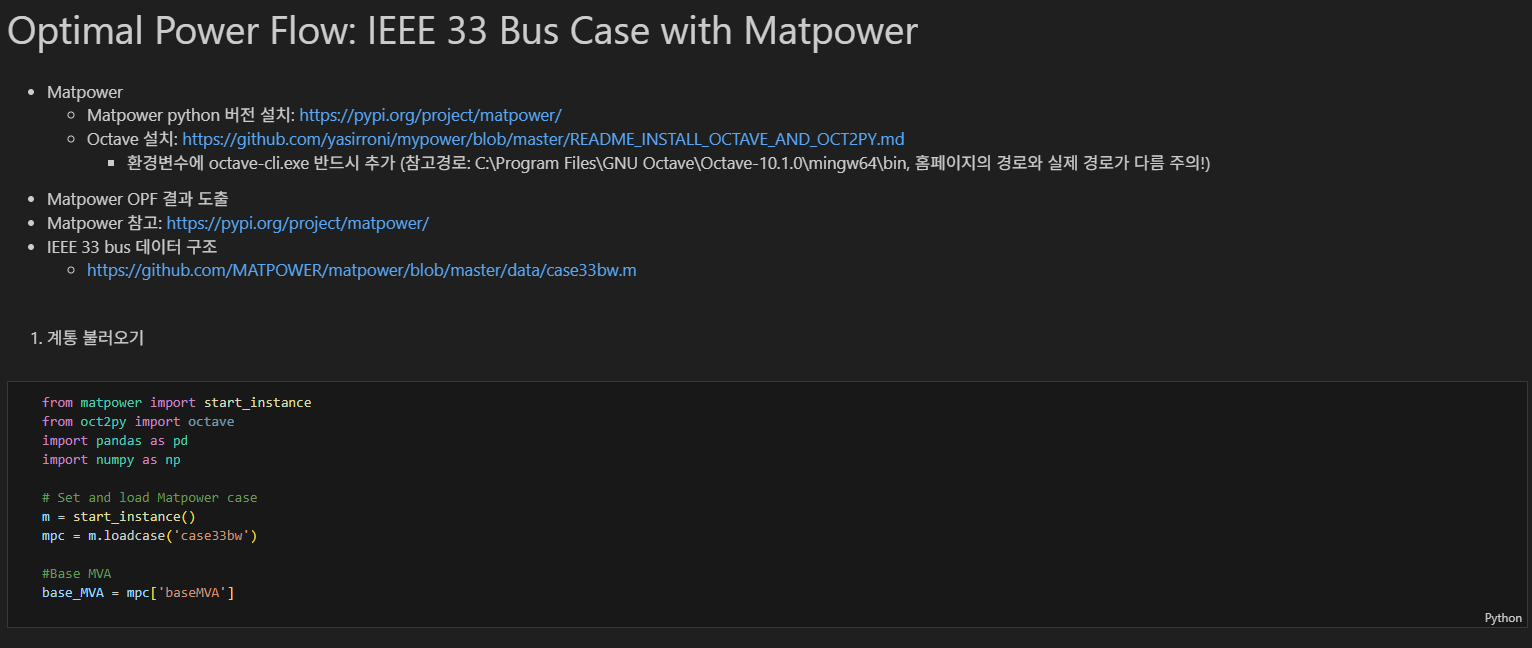
\includegraphics[width=4 in,keepaspectratio]{matpower.png}
	\end{figure}

	
\end{frame}

%------------------------------------------------

\begin{frame}
	\frametitle{Matpower and Pyomo}
	Pyomo can design and solve the optimization problem in python...

	\begin{figure}
		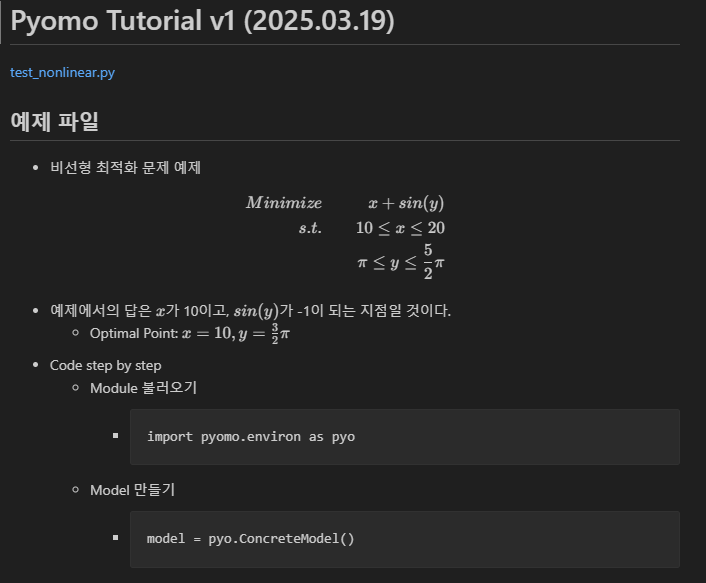
\includegraphics[width=3 in,keepaspectratio]{pyomo.png}
	\end{figure}

\end{frame}

%------------------------------------------------
\subsection{Implementation procedures}
\begin{frame}
	\frametitle{Implementation procedures}
	
	\begin{algorithm}[H]
		\footnotesize % 글자 크기 축소
		\caption{Optimal Power Flow Implementation in Matpower and Pyomo}
		\textbf{Input}: IEEE test system (e.g., case33) \\
		\textbf{Output}: Optimization results (Bus voltage, active/reactive power)
	
	\begin{columns}[T]
		\begin{column}{0.48\textwidth}	
			\begin{enumerate}
			\item Load IEEE test system in Matpower:
			\begin{itemize}
				\item Use the IEEE test system (4,33,...)
			\end{itemize}

			\item Extract parameters from system...:
			\begin{itemize}
				\item Base MVA, slack bus
				\item Bus: \texttt{Vmin/Vmax}
				\item Line: \texttt{R/X}, tap ratio
				\item Generator: \texttt{Pmin/Pmax}, cost
				\item Load data
				\item Build Y-bus
			\end{itemize}

			\end{enumerate}
		\end{column}
		
		\begin{column}{0.48\textwidth}
			\begin{enumerate}
    		\setcounter{enumi}{2}
			
			\item Formulate OPF model:
				\begin{itemize}
					\item Sets, parameters, variables...
					\item Objective: Minimize loss
				\end{itemize}

			\item Solve with Pyomo:
			\begin{itemize}
				\item Select solver (Ipopt,neos,...)
				\item Execute
			\end{itemize}

			\item Save results:
			\begin{itemize}
				\item Voltage profiles
				\item Generation dispatch
			\end{itemize}
		\end{enumerate}
		\end{column}
	\end{columns}
	
	\end{algorithm}
	

\end{frame}

%------------------------------------------------

\subsection{Including Code}
\begin{frame}[fragile]
	\frametitle{Including Code}

	\rule{\textwidth}{1pt}
	
	\rule{\textwidth}{1pt}

\end{frame}
	
%------------------------------------------------


\section{References}

%------------------------------------------------

\begin{frame} % Use [allowframebreaks] to allow automatic splitting across slides if the content is too long
	\frametitle{References}
	
	\printbibliography
	
	
\end{frame}

%----------------------------------------------------------------------------------------
%	ACKNOWLEDGMENTS SLIDE
%----------------------------------------------------------------------------------------

\begin{frame}
	\frametitle{Acknowledgements}
	
	\begin{columns}[t] % The "c" option specifies centered vertical alignment while the "t" option is used for top vertical alignment
		\begin{column}{0.45\textwidth} % Left column width
			\textbf{CWNU Power System Economis Lab}
			\begin{itemize}
				\item Woong Ko
			\end{itemize}
			
		\end{column}		
		
	\end{columns}
\end{frame}

%----------------------------------------------------------------------------------------
%	CLOSING SLIDE
%----------------------------------------------------------------------------------------

\begin{frame}[plain] % The optional argument 'plain' hides the headline and footline
	\begin{center}
		{\Huge The End}
		
		\bigskip\bigskip % Vertical whitespace
		
		{\LARGE Questions? Comments?}
	\end{center}
\end{frame}

%----------------------------------------------------------------------------------------

\end{document} 